\documentclass[a4paper,12pt]{article}
\usepackage{graphicx}
\usepackage{float}
\usepackage{titling}

\setlength{\droptitle}{-14em}
\title{Temperature Autocorrelation Analysis}
\author{PU ZHAO}
\date{\today}

\begin{document}

\maketitle
\section{Results}

\subsection{Correlation Coefficient Calculation}
  \begin{figure}[ht]
    \centering
    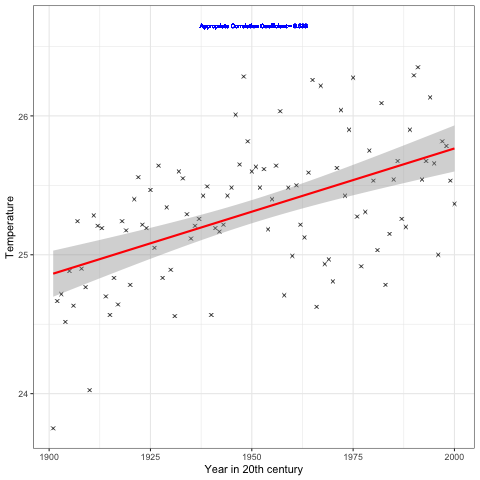
\includegraphics[width=0.7\textwidth]{../data/ats_plot.png}
    \caption{Temperature between consecutive years}
  \end{figure}
  The original correlation coefficient between temperatures of successive years is 0.3261697. It can also be seen from the figure that the correlation between temperatures in consecutive years is not strong.

\subsection{Random Time Series Multiple Calculations}
  \begin{figure}[ht]
    \centering
    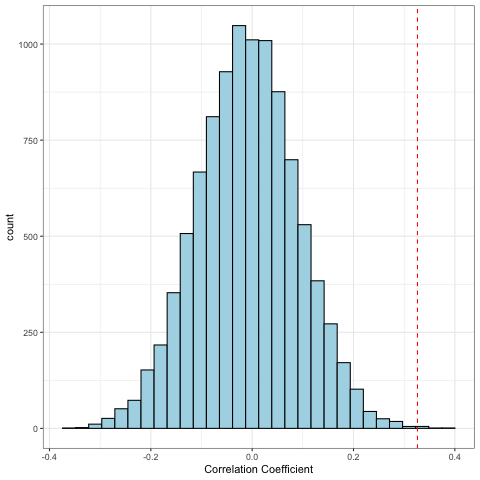
\includegraphics[width=0.7\textwidth]{../data/ats_random_plot.png}
    \caption{Statistical distribution and count of correlation coefficients.}
  \end{figure}
  Through $10,000$ random permutations, it can intuitively observe from the graph that the vast majority of the test correlation coefficients are distributed around 0. The red dashed line in the graph represents the correlation coefficient from the initial test without random event sequencing. It is evident that almost all the test correlation coefficients are greater than the initial correlation coefficient. This also indicates that there is a correlation between the initial temperature and the time series.
\end{document}
